\documentclass[11pt,a4paper]{article}
\usepackage[top=3cm, bottom=2cm, left=2cm, right=2cm]{geometry}
\usepackage[utf8]{inputenc}
\usepackage{amsmath, amsfonts, amssymb}
\usepackage{siunitx}
\usepackage[brazil]{babel}
\usepackage{graphicx}
\usepackage[margin=10pt,font={small, it},labelfont=bf, textfont=it]{caption}
\usepackage[dvipsnames, svgnames]{xcolor}
\DeclareCaptionFont{MediumOrchid}{\color[svgnames]{MediumOrchid}}
\usepackage[pdftex]{hyperref}
\usepackage{natbib}
\bibliographystyle{plainnat}
\bibpunct{[}{]}{,}{s}{}{}
\usepackage{color}
\usepackage{footnote}
\usepackage{setspace}
\usepackage{booktabs}
\usepackage{multirow}
\usepackage{subfigure}
\usepackage{fancyhdr}
\usepackage{leading}
\usepackage{indentfirst}
\usepackage{wrapfig}
\usepackage{mdframed}
\usepackage{etoolbox}
\usepackage[version=4]{mhchem}
\usepackage{enumitem}
\usepackage{caption}
\usepackage{titlesec}
\usepackage{tcolorbox}
\usepackage{tikz}
\usepackage{LobsterTwo}
\usepackage[T1]{fontenc}
\usepackage{fontspec}
\usepackage{txfonts}
\AtBeginEnvironment{equation}{\fontsize{13}{16}\selectfont}


\titleformat{\section}{\LobsterTwo\LARGE\color{CarnationPink}}{\thesection.}{1em}{}
\titleformat{\subsection}{\LobsterTwo\LARGE\color{CarnationPink}}{\thesubsection}{1em}{}
\titleformat{\subsubsection}{\LobsterTwo\Large\color{CarnationPink}}{\thesubsubsection}{1em}{}


\DeclareCaptionLabelFormat{figuras}{\textcolor{DarkTurquoise}{Figura \arabic{figure}}}
\captionsetup[figure]{labelformat=figuras}

\makeatletter
\renewcommand\tagform@[1]{\maketag@@@{\color{CarnationPink}(#1)}}
\makeatother

\renewcommand{\theequation}{Eq. \arabic{equation}}
\renewcommand{\thefigure}{Fig. \arabic{figure}}
\renewcommand{\thesection}{\textcolor{CarnationPink}{\arabic{section}}}

\setlist[itemize]{label=\textcolor{CarnationPink}{$\mathbf{\square}$}}

\setlist[enumerate]{label=\textcolor{CarnationPink}{\arabic*.}, align=left}


\newcounter{exemplo}

\NewDocumentEnvironment{exemplo}{ O{} }{%
\allowbreak
\setlength{\parindent}{0pt}
  \begin{mdframed}[
  leftline=true,
  topline=false,
  rightline=false,
  bottomline=false,
  linewidth=2pt,
  linecolor=CarnationPink,
  frametitlerule=false,
  frametitlefont=\LobsterTwo\large\color{CarnationPink},
  frametitle={\color{CarnationPink}\LobsterTwo\large #1},
  ]
}{%
  \end{mdframed}
}

\setlength{\fboxsep}{5pt}
\setlength{\fboxrule}{1.5pt}
\usepackage{float}
\renewcommand{\thefootnote}{\alph{footnote}}
\usepackage{url}
\hypersetup{
	colorlinks=true,
	linkcolor=DarkTurquoise,
	filecolor=DarkTurquoise,      
	urlcolor=DarkTurquoise,
	citecolor=DarkTurquoise,
	pdftitle={Especialista em Física da Radioterapia}
}
\pagestyle{fancy}
\fancyhf{}
\renewcommand{\headrulewidth}{0pt}
\rfoot{Página \thepage}

\title{\LobsterTwo\Huge{Braquiterapia}}
\author{\LobsterTwo\Large{Braquiterapia Intracavitária}\nocite{*}}
\date{\LobsterTwo\textit{Dalila Mendonça}}
\begin{document}
	\maketitle

\section{Introdução}

	A braquiterapia intracavitária pode ser realizada usando fontes de baixa taxa de dose (LDR), taxa de dose pulsada (PDR) ou alta taxa de dose (HDR). Os implantes LDR expõem a equipe de atendimento ao paciente a mais radiação do que o HDR e requerem um tempo de internação mais longo do paciente e mais recursos dedicados ao armazenamento da fonte e medidas de radioproteção. Há também um risco aumentado de erro, por exemplo, selecionando a força da fonte incorreta ao recuperar as cápsulas da fonte do armazenamento ou implantar as fontes na ordem incorreta. Por esses motivos, a braquiterapia intracavitária mudou amplamente para a administração HDR usando afterloaders remotos.

	O principal problema na transição da LDR para HDR foi em estabelecer regimes de fracionamento de dose equivalentes. A LDR tinha uma longa história clínica com fracionamento da dose bem estabelecido, taxas de sobrevivência e taxas de complicações. Teoricamente, a HDR tem uma razão terapêutica menor que a LDR devido à curta duração dos tratamentos. O tratamento HDR com planejamento de tratamento computadorizado tem a capacidade de otimizar a dose entregue nos alvos e estruturas críticas, o que pode superar esse déficit biológico. De fato, estudos mostraram a equivalência de LDR e HDR.

	Ao avaliar tratamentos de HDR, às vezes é útil converter a dose para doses radiobiologicamente equivalentes (mais comumente o EQD2, ou dose equivalente em frações de 2 Gy dia), embora seja importante lembrar as advertências e suposições que acompanham essas conversões baseadas em modelos teóricos.  Numerosas calculadoras de dose biologicamente equivalente (BED) estão disponíveis online e como aplicativos; a American Brachytherapy Society (ABS) fornece planilhas do Excel para converter doses de HDR em doses equivalentes a 2 Gy (\href{http://www.americanbrachytherapy.org/guidelines/index.cfm}{http://www.americanbrachytherapy.org/guidelines/index.cfm}).

\section{Sítios de Tratamento}

	A braquiterapia intracavitária aproveita as vias anatômicas para colocar fontes radioativas diretamente adjacentes aos locais do tumor. Isso é menos invasivo do que os implantes intersticiais e pode, em muitos casos, ser feito sem anestesia geral.

	Os aplicadores ginecológicos padrão (gyn) são feitos de aço cirúrgico com plásticos utilizados como capas de buildup e como segmentos de cilindros vaginais. Aplicadores compatíveis com ressonância magnética (MRI) substituem o aço cirúrgico por titânio ou fibra de carbono; nenhum desses materiais tem a mesma resistência mecânica do aço cirúrgico e, portanto, requerem cuidados redobrados no manuseio durante a esterilização e durante o procedimento.

\subsection{Sítios Ginecológicos}

\subsubsection*{Endométrio}

	Uma aplicação comum da braquiterapia intracavitária é o tratamento de câncer endometrial. A Figura 20.1 mostra a anatomia para referência. As diretrizes de consenso da ABS para braquiterapia de manguito vaginal\footnote{O "vaginal cuff" é o termo em inglês usado para descrever a área da vagina após a remoção do colo do útero durante uma histerectomia. Durante a cirurgia, o colo do útero é removido e a parte superior da vagina é suturada, criando uma espécie de "cuff" ou manguito vaginal.} adjuvante após histerectomia contêm as recomendações mais recentes da sociedade sobre esse procedimento.

	\begin{figure}[h]
		\centering
		\subfigure[Anterior]{
		\fcolorbox{DarkTurquoise}{white}{%
			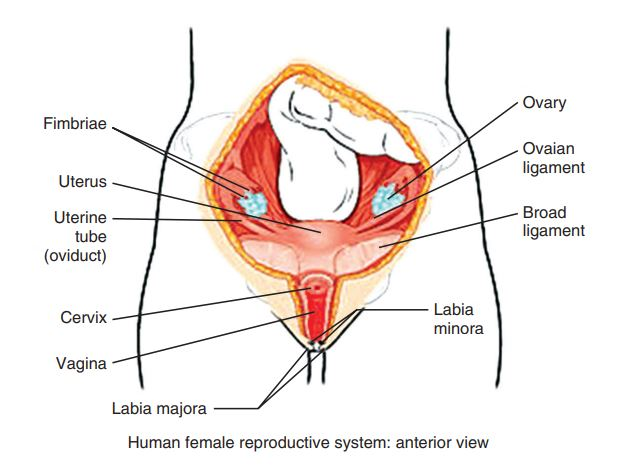
\includegraphics[width=0.46\textwidth]{Imagens/AnatomiaGinecoAnterior.JPG}
		}}%
		\subfigure[Lateral]{
		\fcolorbox{DarkTurquoise}{white}{%
			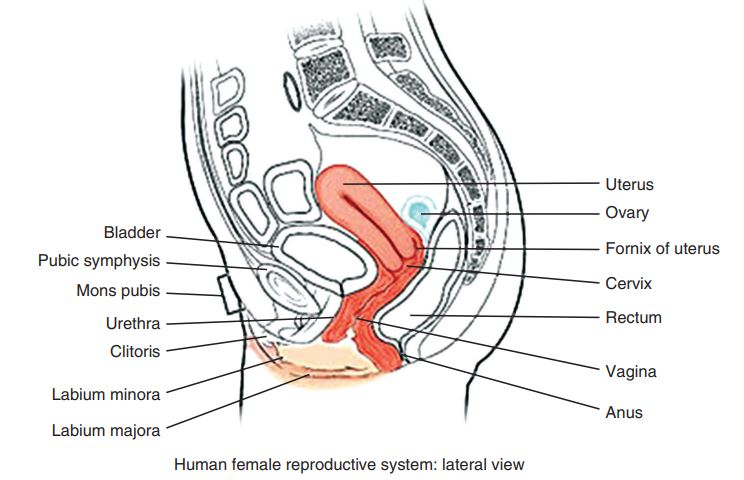
\includegraphics[width=0.52\textwidth]{Imagens/anatomiaGinecoLateral.JPG}
		}} \\ %
		\caption{Anatomia da vagina, colo do útero e útero.}
		\label{fig:AnatomiaGineco}
	\end{figure}

	De acordo com as diretrizes da National Comprehensive Cancer Network (NCCN), para pacientes em estágio I sem fatores de risco adversos, a braquiterapia pode ser a única terapia adjuvante após a cirurgia. Para pacientes em estágio I com fatores de risco adversos e pacientes em estágio II, a teleterapia da pelve com uma dose de 4500 cGy a 5000 cGy é administrada além da braquiterapia.

	Após a remoção cirúrgica do útero, o aplicador padrão é um cilindro segmentado com um cateter central. Um conjunto de cilindros padrão consiste em cilindros de diferentes diâmetros (2 cm a 4 cm) com vários segmentos cada e um ou dois tipos de capas de cilindro. O médico escolhe o cilindro adequado com base na anatomia do paciente; o objetivo é usar a forma cilíndrica que minimiza quaisquer gaps de ar entre o cilindro e o tecido. Na prática, é usado o cilindro de maior diâmetro possível de modo que seja confortável para a paciente. Isso tem o benefício adicional de reduzir a taxa de queda de dose além do cilindro devido à lei do quadrado inverso. A \ref{fig:implanteCilindro} mostra um implante de cilindro típico.

	\begin{figure}[h]
		\centering
		\fcolorbox{DarkTurquoise}{white}{%
			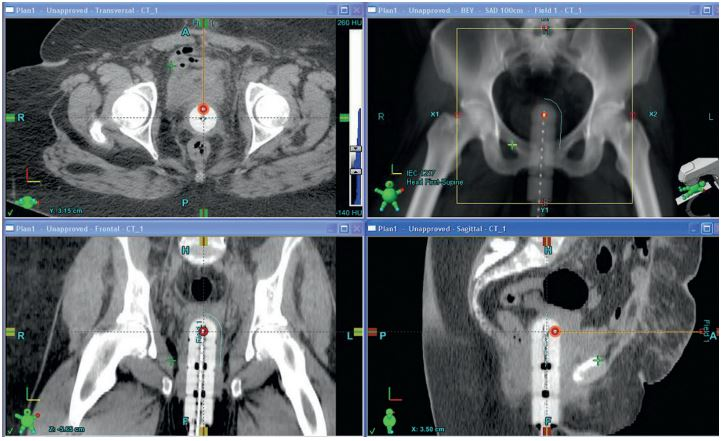
\includegraphics[width=0.4\textwidth]{Imagens/implanteCilindro.JPG}
		}%
		\caption{Implante de cilindro HDR típico.}
		\label{fig:implanteCilindro}
	\end{figure}

	Uma variação do cilindro padrão é o cilindro blindado, no qual segmentos de blindagem de tungstênio de \ang{90}, \ang{180} e \ang{270} podem ser inseridos. Os cilindros blindados têm a desvantagem de que a imagem de tomografia de simulação para o planejamento do tratamento não pode ser obtida com as blindagens em suas posições devido aos grandes artefatos que a blindagem causaria. Alguns aplicadores blindados têm blindagens removíveis para que possam ser colocadas após a aquisição das imagens. 
	
	Como uma solução para os desafios de aquisição de imagem que acompanham os cilindros blindados, o aplicador Miami foi projetado para permitir a distribuição de dose não cilíndrica sem o uso de blindagens de metal. Seu design é semelhante a um cilindro, mas além do canal central, seis canais periféricos permitem a customização da distribuição da dose. A maioria dos design de cilindros e aplicadores Miami permitem que o canal central seja substituído por um tandem (sonda) para tratar pacientes clinicamente inoperáveis, nas quais o útero não foi removido. A \ref{fig:cilindros} mostra os aplicadores cilíndricos típicos. Um aplicador tandem e ovoide também pode ser usado para esses pacientes. Mais recentemente, a tecnologia de impressão 3D foi usada para imprimir aplicadores de cilindro personalizados e um cilindro vaginal inflável foi introduzido.
	
	\begin{figure}[h]
		\centering
		\subfigure{
		\fcolorbox{DarkTurquoise}{white}{%
			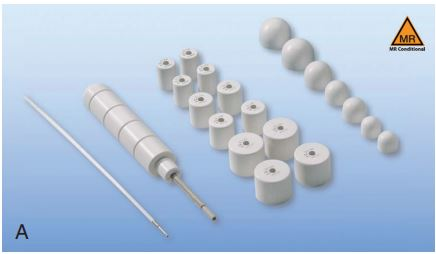
\includegraphics[width=0.4\textwidth]{Imagens/cilindroSegmentado.JPG}
		}}%
		\subfigure{
		\fcolorbox{DarkTurquoise}{white}{%
			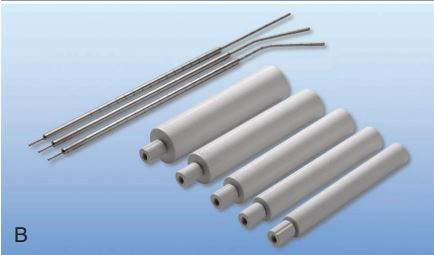
\includegraphics[width=0.4\textwidth]{Imagens/aplicadorCervix.JPG}
		}} \\ %
		\subfigure{
		\fcolorbox{DarkTurquoise}{white}{%
			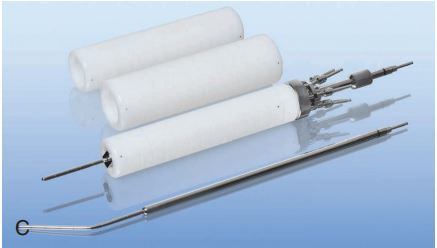
\includegraphics[width=0.4\textwidth]{Imagens/aplicadorMiami.JPG}
		}}%
		\subfigure{
		\fcolorbox{DarkTurquoise}{white}{%
			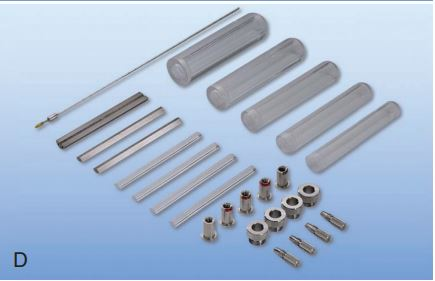
\includegraphics[width=0.4\textwidth]{Imagens/aplicadorBlindado.JPG}
		}} \\ %
		\caption{Aplicadores Cilíndricos: \textbf{A}, Conjunto aplicador de cilindro segmentado (Varian Medical Systems). \textbf{B}, Conjunto aplicador de colo do útero (Varian Medical Systems). \textbf{C}, Conjunto de aplicadores estilo Miami (Varian Medical Systems). \textbf{D}, Conjunto aplicador blindado (Varian Medical Systems).}
		\label{fig:cilindros}
	\end{figure}

\subsubsection*{Colo de Útero}

	Os guidelines da ABS para carcinoma localmente avançado do colo do útero, Parte I Geral e Parte II HDR, abrangem a avaliação pré-tratamento, o tratamento e questões dosimétricas para o tratamento do câncer de colo de útero localmente avançado. O guideline também recomendam a adoção dos guidelines da ``Groupe Europeen Curietherapie European Society of Therapeutic Radiation Oncology (GEC-ESTRO)'' para contorno, planejamento de tratamento utilizando imagens e reports de dose.

	Exceto para o câncer de endométrio em estágio muito inicial (FIGO IA-IB1), a braquiterapia é administrada diretamente após a teleterapia (EBRT) ou em conjunto com a EBRT (4 frações de EBRT e 1 fração de braquiterapia por semana). A dose da teleterapia é geralmente em torno de 4500 cGy, enquanto a dose de HDR é tipicamente de 550 cGy a 600 cGy por fração totalizando cinco frações. A duração total do tratamento não deve exceder 8 semanas, incluindo a braquiterapia.

	Para o tratamento do câncer cervical, o aplicador intracavitário clássico é o tandem e ovoides (T\&O). O tandem é inserido através do orifício cervical no útero. Os dois ovóides (ou colpostatos) são colocados lateralmente nos fórnices vaginais. A \ref{fig:implanteOvoide} mostra um implante T\&O típico.

	\begin{figure}[h]
		\centering
		\subfigure{
		\fcolorbox{DarkTurquoise}{white}{%
			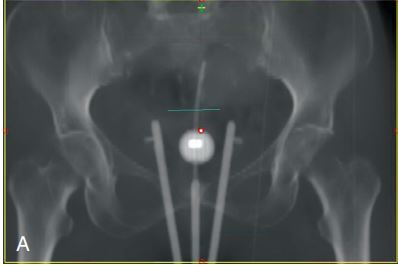
\includegraphics[width=0.4\textwidth]{Imagens/implanteOvoideAnterior.JPG}
		}} \\ %
		\subfigure{
		\fcolorbox{DarkTurquoise}{white}{%
			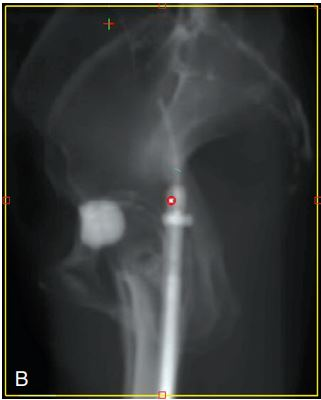
\includegraphics[width=0.4\textwidth]{Imagens/implanteOvoideLateral.JPG}
		}}%
		\caption{\textbf{A}, imagem AP de um implante tandem e ovoide. \textbf{B}, Imagem lateral de um implante tandem e ovoide.}
		\label{fig:implanteOvoide}
	\end{figure}

	Os conjuntos de aplicadores T\&O vêm com uma variedade de sondas de vários comprimentos e ângulos de curvatura de \ang{30}, \ang{45} e \ang{60}. As capas dos ovóides, cuja finalidade é remover o tecido cervical de regiões com dose muito alta, vêm em diferentes diâmetros para serem personalizáveis de acordo com a anatomia do paciente. Capas de ovóides blindadas também estão disponíveis, mas não são usadas com muita frequência. 
	
	Existem vários tipos de aplicadores tandem e ovóides: Os ovóides Fletcher e Fletcher-Suit-Delclos orientam as posições de parada em uma direção principalmente anterior/posterior. Os ovóides de Henschke e Manchester orientam as posições de parada em uma direção inferior/superior. Uma variação do aplicador T\&O é o aplicador tandem e anel (T\&R), no qual os ovóides são substituídos por um anel. A \ref{fig:aplicadoresCervix} mostra aplicadores típicos utilizados na braquiterapia de colo de útero.

	\begin{figure}[h]
		\centering
		\subfigure{
		\fcolorbox{DarkTurquoise}{white}{%
			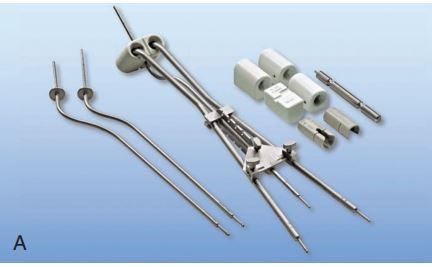
\includegraphics[width=0.4\textwidth]{Imagens/fletcher.JPG}
		}} %
		\subfigure{
		\fcolorbox{DarkTurquoise}{white}{%
			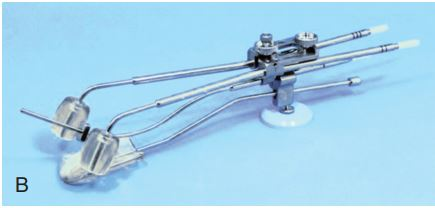
\includegraphics[width=0.4\textwidth]{Imagens/fletcherMick.JPG}
		}} \\ %
		\subfigure{
		\fcolorbox{DarkTurquoise}{white}{%
			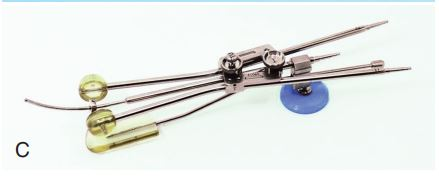
\includegraphics[width=0.4\textwidth]{Imagens/henscke.JPG}
		}} %
		\subfigure{
		\fcolorbox{DarkTurquoise}{white}{%
			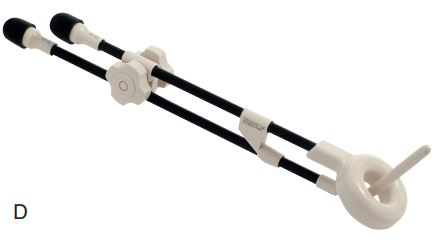
\includegraphics[width=0.4\textwidth]{Imagens/aneleSonda.JPG}
		}} \\ %
		\caption{\textbf{A}, geometria definida do aplicador estilo Fletcher (Varian Medical
		Sistemas). \textbf{B}, aplicador Fletcher-Suit-Delclos (Mick Radio-Nuclear Instruments). \textbf{C}, aplicador Henschke (Mick Radio-Nuclear Instruments). \textbf{D}, Aplicador anel e tandem (Elekta AB).}
		\label{fig:aplicadoresCervix}
	\end{figure}

	O anel também é possui uma capa, semelhante aos ovóides. A vantagem do anel é que este aplicador é mais fácil de colocar, especialmente para pacientes com orifício cervical raso, quando comparado aos ovóides. Para tumores unilateralmente volumosos, é mais difícil obter uma boa colocação do anel, e um T\&O (ligeiramente assimétrico) pode ser a melhor escolha. Para doença volumosa (\textit{``bulky''}), os aplicadores T\&O/T\&R às vezes são complementados com a adição de duas a três agulhas intersticiais usando implantes de agulha à mão livre (sem template). Também estão disponíveis aplicadores combinados de T\&O/T\&R com um número limitado de agulhas intersticiais embutidas no aplicador. Os aplicadores T\&O/T\&R também possuem um afastador retal, que é utilizado para aumentar a distância entre o implante e o reto. O espaço entre o afastador retal e o aplicador é preenchido com gaze úmida (tamponamento). O tamponamento também é colocado anteriormente para ajudar a reduzir as doses na bexiga.

	Um bom tamponamento e a obtenção de uma boa geometria são fundamentais para a obtenção de um implante de alta qualidade. Para alcançar uma alta qualidade no implante, os ovóides ou anel precisam estar o mais próximo possível do orifício cervical no sentido superior, mas o mais lateralmente possível em relação à sonda. Isto é feito para que a distância do ovoide ou do anel até o ponto ou volume de prescrição seja menor do que a distância dos seus pontos de parada até o reto.

	Se as posições de parada dos ovóides estiverem posicionadas muito perto da linha média definida pela sonda, é mais provável que os ovóides administrem uma dose mais alta perto do reto. Se for esse o caso, a contribuição para dose no reto devido as posição de parada dos ovóides será sempre maior que a contribuição para a dose no ponto de prescrição, dificultando muito a obtenção de uma boa distribuição de dose. O afastador retal e o tamponamento podem ajudar a afastar o reto dos ovóides e do anel, mas também é aconselhável obter uma boa geometria mesmo utilizando esses recursos. Para mulheres com fórnice\footnote{O fórnice é a região de encontro do canal vaginal com o colo do útero. É a porção mais profunda da vagina} estreito, pode ser muito difícil alcançar uma boa geometria. Nestes casos, às vezes, um cilindro vazado com o tandem pode ser uma opção.

	Os guidelines da ABS para carcinoma localmente avançado do colo do útero, Parte I Geral, definem os seguintes critérios para um implante adequado:

	\begin{itemize}[label=\textcolor{CarnationPink}{$\blacksquare$}]
		\item O tandem deve ser centralizado entre os ovóides em uma imagem ântero-posterior (AP) e interceptá-los em uma imagem lateral.
		\item Em uma imagem lateral, os ovóides não devem ser deslocados inferiormente ao flange (presilha que define a profundidade com base a histerometria) e devem ser o mais simétricos possível (devem se sobrepor).
		\item O tandem deve ter aproximadamente metade a um terço da distância entre a sínfise púbica e o promontório sacral, e estar aproximadamente equidistante entre uma bexiga cheia de contraste e o reto.
		\item A ponta superior do tandem deve estar localizada abaixo do promontório sacral dentro da pelve. 
		\item O tamponamento com gaze radiopaca ou utilização de retratores retais  deverão visível nas imagens radiográficas e devem ser colocado anterior e posteriormente aos ovóides, sem nenhum tamponamento visível superior aos ovóides. O tamponamento superior representa um deslocamento inferior indesejado do aplicador e indica a necessidade de refazer o tamponamento adequadamente antes do carregamento da fonte.
	\end{itemize}
	
\subsubsection*{Câncer Vaginal}

	O tratamento para os cânceres vaginais é semelhante ao dos cânceres de endométrio, pois também é usado um cilindro vaginal. Se a doença estiver confinada a uma área limitada, pode ser usado um cilindro blindado.

\subsubsection*{Cavidade Uterina}

	Para o tratamento de toda cavidade uterina em pacientes inoperáveis em Estágio I, um tandem sozinho não seria capaz de fornecer uma boa cobertura de dose. Uma solução foi o uso de cápsulas de Heyman, que consistiam em várias cápsulas de baixa dose de \ce{^{137}Cs} acondicionadas no útero. Originalmente, a dose foi estimada com base no número de cápsulas e no tempo de tratamento, mas nenhum cálculo preciso da dose estava disponível. Com o advento do planejamento de tratamento computadorizado, cálculos de dose foram realizados. As cápsulas de Heyman também estavam disponíveis no formato afterloading para uso com \ce{^{192}Ir}. As cápsulas de Heyman foram substituídas por aplicadores Y, que consistem em dois tandems montados em um aplicador com as pontas tandem inclinadas uma da outra na forma de um Y. Como os tandems únicos, os tandems duplos para os aplicadores Y vêm em uma variedade de tamanhos e ângulos. Além disso, às vezes é usado um tandem central reto (sonda reta). A Figura 20.6 mostra um conjunto de aplicador típico. Atualmente, o planejamento utilizando imagens 3D de TC ou RM é feito para identificar com precisão o volume alvo e as estruturas críticas.

	\begin{figure}[h]
		\centering
		\subfigure{
			\fcolorbox{DarkTurquoise}{white}{%
				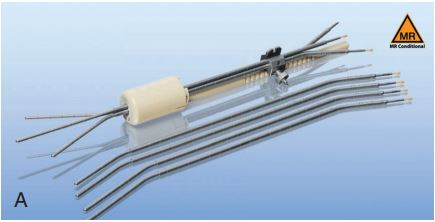
\includegraphics[width=0.43\textwidth]{Imagens/endometrioUniversalAplicador.JPG}
			}} %
		\subfigure{
			\fcolorbox{DarkTurquoise}{white}{%
				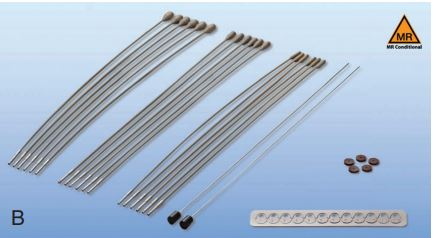
\includegraphics[width=0.4\textwidth]{Imagens/heymanpacking.JPG}
			}} %
		\caption{\textbf{A}, Conjunto de aplicador endometrial universal (Varian Medical Systems). \textbf{B}, Conjunto aplicador Heyman (Varian Medical Systems).}
		\label{fig:heyman}
	\end{figure}
	
\subsection{Tratamentos Endobronquiais, Esofágicos e Nasofaríngeo}

	Tumores na árvore brônquica, esôfago e nasofaringe também podem ser tratados com braquiterapia intracavitária. Um único cateter é inserido com auxílio de imagens fluoroscópica um pouco além da localização do tumor. O comprimento do cateter é medido e deve ser cuidadosamente verificado antes de cada tratamento esofágico ou nasofaríngeo. Para tratamentos endobrônquicos, o cateter é colocado o mais abaixo possível na via aérea para ancorá-lo no lugar. Se isso não for feito, o cateter pode se deslocar se o paciente tossir.A distribuição da dose geralmente tem simetria cilíndrica e, devido ao uso de apenas um canal, há uma limitada flexibilidade na configuração da dose. 
	
	Lesões endobrônquicas próximas à carina podem exigir dois canais, cada um descendo para um brônquio principal. O ponto de prescrição para tratamentos endobrônquicos pode variar. Geralmente o ponto de prescrição é determinado a 5 mm do centro do cateter. Porém, as vias aéreas principais podem ser significativamente maiores do que 5 mm de raio e, portanto, às vezes o ponto de prescrição é definido a 10 mm do centro do cateter. A dificuldade em usar distâncias de prescrição maiores é que o cateter não fica centralizado na via aérea, mas sim apoiado em uma parte da parede da via aérea, de modo que prescrever a dose para 10 mm pode fazer com que partes da parede recebam dose excessiva.

	Os cateteres foram projetados com mecanismos de centralização retráteis para combater esse efeito. Isso aponta uma das principais falhas dos tratamentos endobrônquicos. O cateter está confinado às vias aéreas e, portanto, apenas pequenas lesões podem ser tratadas, porque deslocar a dose para fora para tratar lesões maiores causaria uma dose excessiva na parede das vias aéreas. Por esse motivo, a braquiterapia intracavitária nessas regiões foi amplamente substituída por abordagens de radioterapia de intensidade modulada (IMRT) ou, às vezes, terapia fotodinâmica. As diretrizes de consenso da ABS para braquiterapia de câncer de esôfago fornecem detalhes sobre a seleção de pacientes, regimes de fracionamento de dose para braquiterapia definitiva, adjuvante e paliativa e seleção de aplicadores.

\subsection{Reto}

	O desenvolvimento mais recente em aplicadores intracavitários é o desenvolvimento de aplicadores retais. Novos desenvolvimentos em materiais, aplicadores de uso único e imagens 3D para planejamento de tratamento foram as pré-condições necessárias para facilitar a implementação clínica. Devido à proximidade de estruturas críticas e à própria sensibilidade à radiação, esforços estão em andamento para desenvolver aplicadores retais que permitam a blindagem seletiva de áreas que não precisam ser tratadas. A \ref{fig:aplicadorReto} mostra o aplicador intracavitário para o reto chamado de Mold, que cosiste em oito cateteres espaçados radialmente, posicionados na superfície do cilindro que permitem carregamento diferencial para garantir melhor cobertura do alvo e proteção dos tecidos circunvizinhos. Existe uma abertura central que pode ser utilizada como um cateter ou pode ser utilizada para inserir as blindagens. 

	\begin{figure}[h]
		\centering
		\fcolorbox{DarkTurquoise}{white}{%
			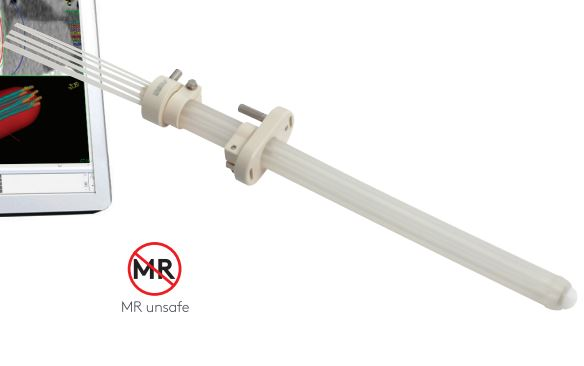
\includegraphics[width=0.4\textwidth]{Imagens/aplicadorReto.JPG}
		}%
		\caption{Intracavitary Mold Applicator (Elekta) para tratamentos de reto. }
		\label{fig:aplicadorReto}
	\end{figure}

\section{Planejamento de Tratamento}

\subsection*{Aquisição das Imagens}

	Os guidelines da ABS para carcinoma localmente avançado do colo do útero, recomendam o uso de imagens em cortes transversais (TC ou RM). Embora a RM tenha um melhor contraste para visualização de tecidos moles, fornecendo uma melhor informação a respeito da extensão do tumor e o envolvimento parametrial, as imagens de TC estão mais amplamente disponíveis. Também podem ser utilizadas imagem PET para avaliar o envolvimento nodal. 
	
	Todos os equipamentos de imagem dedicados à Braquiterapia devem passar por controle de qualidade periódico para garantir precisão espacial e transferência correta das imagens para o TPS. Com base em pesquisas realizadas em 2010, aproximadamente 55\% dos praticantes de braquiterapia usam imagens de TC para simulação do tratamento (O que está MUITO longe de ser uma realidade aqui no Brasil). 

\subsection*{Contorno e Pontos de Análise de Dose}

	O planejamento do tratamento deve levar em consideração a dose fornecida pelos componentes da radioterapia externa e da braquiterapia. As prescrições de dose devem seguir as regras para diretivas escritas estabelecidas e conter informações sobre o isótopo e a configuração da fonte, alvo, dose alvo e fracionamento e tipo de aplicador. As restrições de dose para órgãos de risco (OARs) também devem ser listadas.

\subsection*{ICRU-38}

	O ICRU-38, \textit{``Dose and Volume Specification for Reporting Intracavitary Therapy in Gynecology''}, publicado em 1985, utilizava um método de prescrição de dose que, mesmo na época, era pouco utilizado. A prescrição de dose usa as três dimensões máximas da superfície de isodose de 60 Gy (menos qualquer dose fornecida por feixe externo). O comprimento máximo é medido com base no plano que contém o tandem, enquanto a largura máxima é medida perpendicularmente à medida da altura, geralmente na altura dos ovóides, como mostra a \ref{fig:icru38Presc} .

	\begin{figure}[h]
		\centering
		\subfigure{
			\fcolorbox{DarkTurquoise}{white}{%
				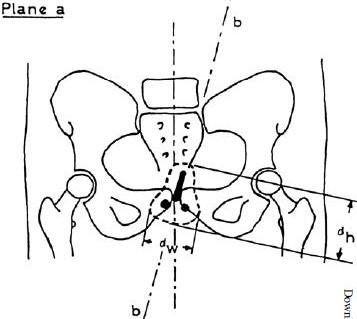
\includegraphics[width=0.30\textwidth]{Imagens/icru38A.JPG}
		}} %
		\subfigure{
			\fcolorbox{DarkTurquoise}{white}{%
				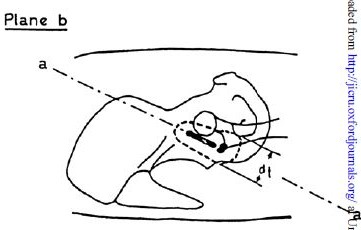
\includegraphics[width=0.40\textwidth]{Imagens/icru38B.JPG}
		}} \\ %
		\caption{Geometria para medida do tamanho da superfície de isodose de 60 Gy em forma de pêra (linha tracejada) em um tratamento típico de carcinoma de colo uterino usando um aplicador uterino em forma de bastonete e 2 aplicadores vaginais. O plano a é o plano frontal "oblíquo" que contém o dispositivo intrauterino. O plano frontal oblíquo é obtido pela rotação do plano frontal em torno de um eixo transversal, o Plano b é o plano sagital "oblíquo" que contém o dispositivo intrauterino. O plano sagital oblíquo é obtido pela rotação do plano sagital em torno do eixo AP. A altura (db) e a largura (dw) do volume de referência são medidas no plano a como os tamanhos máximos paralelos e perpendiculares ao aplicador uterino, respectivamente. A espessura (dt) do volume de referência é medida no plano b como o tamanho máximo perpendicular ao aplicador uterino.}
		\label{fig:icru38Presc}
	\end{figure}

	O \textcolor{DarkTurquoise}{\textbf{ponto da bexiga}} é definido no trígono da bexiga conforme visualizado por um balão de Foley preenchido com 7 \unit{cm^3}  de contraste diluído. Este ponto geralmente não se correlaciona com a dose máxima na bexiga.
	
	O \textcolor{DarkTurquoise}{\textbf{ponto de reto}} é definido como uma linha vertical diretamente posterior ao centro dos ovóides/anel e a 0.5 cm posterior à parede vaginal posterior. O método mais preciso de visualizar este ponto nas radiografias é com o uso de contraste de bário; marcadores retais de chumbo não são tão confiáveis e reduzirão sistematicamente a dose reportada. Novamente, esse ponto de reto nem sempre coincide com a dose máxima no reto. O ponto de reto e bexiga são esquematizados na \ref{fig:icru38RetoEBexiga}

	\begin{figure}[h]
		\centering
		\fcolorbox{DarkTurquoise}{white}{%
			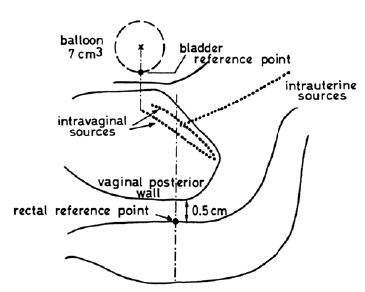
\includegraphics[width=0.4\textwidth]{Imagens/icru38RetoEBexiga.JPG}
		}%
		\caption{Definição do ponto de reto e do ponto de bexiga.}
		\label{fig:icru38RetoEBexiga}
	\end{figure}


	Os \textcolor{DarkTurquoise}{\textbf{pontos da parede pélvica}} são determinados pela interseção das duas linhas na radiografia AP: \textcolor{MediumOrchid}{$\mathbf{(i)}$} a linha que conecta as faces superiores do acetábulo e \textcolor{MediumOrchid}{$\mathbf{(ii)}$} as tangentes às faces mediais do acetábulo que se cruzam em ângulos retos com \textcolor{MediumOrchid}{$\mathbf{(i)}$}. Na radiografia lateral, a posição seria aproximada pelo ponto médio de \textcolor{MediumOrchid}{$\mathbf{(i)}$}, como mostra a \ref{fig:icru38paredePelvica}.

	\begin{figure}[h]
		\centering
		\fcolorbox{DarkTurquoise}{white}{%
			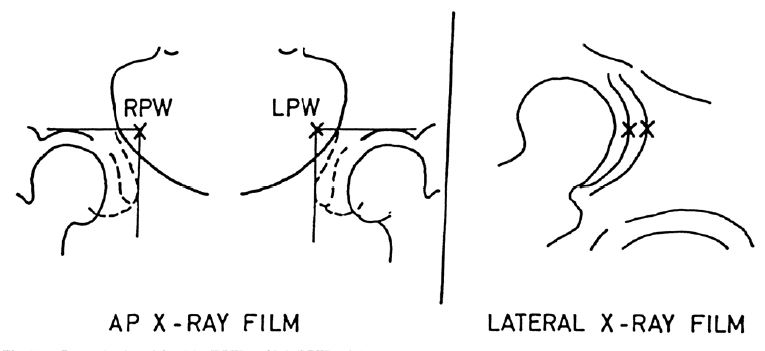
\includegraphics[width=0.6\textwidth]{Imagens/icru38paredePelvica.JPG}
		}%
		\caption{Determinação dos pontos da parede pélvica}
		\label{fig:icru38paredePelvica}
	\end{figure}

\subsection*{Sistema Manchester}

	O sistema de Manchester foi originalmente desenvolvido em meados do século 20 com base nas técnicas de carregamento de fonte mais antigas do sistema de Paris e nos esquemas de fracionamento do sistema de Estocolmo. Este sistema define a prescrição e os pontos de avaliação de dose nos OAR que ainda estão sendo usados hoje para caracterizar implantes T\&O/T\&R e tandem e cilindro (T\&C). A principal novidade do sistema Manchester foi a constatação de que a estrutura anatômica dose-limitante era a área na qual os vasos uterinos cruzam o ureter. Uma vez que esses marcadores anatômicos não podiam ser visualizados nas imagens da época, um método foi desenvolvido para aproximar a posição desses marcadores anatômicos em relação ao aplicador radiopaco que podia ser visto em raios-x ortogonais para uma ampla população de pacientes. O plano de tratamento foi então projetado para fornecer a taxa de dose prescrita nesses pontos, $A_{left}$ e $A_{right}$.

	O \textcolor{DarkTurquoise}{\textbf{ponto A (esquerdo e direito)}} está localizado conforme definido pela recomendação ABS de 2011: \textcolor{MediumOrchid}{\textit{``No TPS, conecte uma linha através do centro de cada ovóide ou a posição de parada mais lateral em um anel. Do ponto no tandem onde esta linha se cruza, estenda superiormente o raio dos ovóides ou para os anéis mova-se superiormente até o topo do anel e depois mova 2 cm ao longo do tandem. Defina o ponto A em cada lado como 2 cm lateralmente em uma linha perpendicular a partir deste ponto no tandem. Para tandem e cilindros, comece no flange ou sementes marcando o orifício do colo uterino e mova 2 cm superiormente ao longo do tandem e 2 cm lateralmente em uma linha perpendicular.''}} Observe que a linha que liga os pontos A é sempre perpendicular ao tandem. Para implantes em que os ovóides/anel são forçados pela anatomia a serem levemente assimétricos em relação ao tandem, os pontos A terão distâncias diferentes das fontes até os ovóides/anel. Na prática clínica, a prescrição de dose é muitas vezes definida como a média das doses nos pontos A. A \ref{fig:pontoA} apresenta a determinação do ponto a para diferentes aplicadores utilizados no tratamento de colo uterino.
	
	\begin{figure}[h]
		\centering
		\subfigure{
			\fcolorbox{DarkTurquoise}{white}{%
				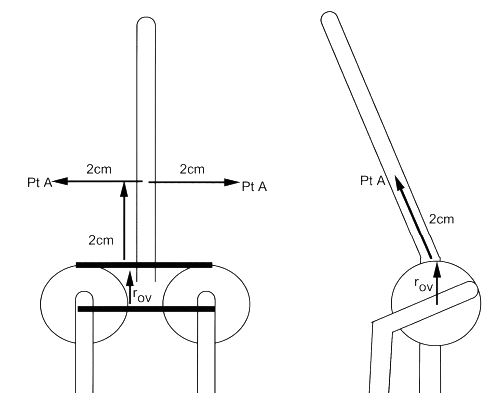
\includegraphics[width=0.4\textwidth]{Imagens/pontoA.JPG}
			}} %
		\subfigure{
			\fcolorbox{DarkTurquoise}{white}{%
				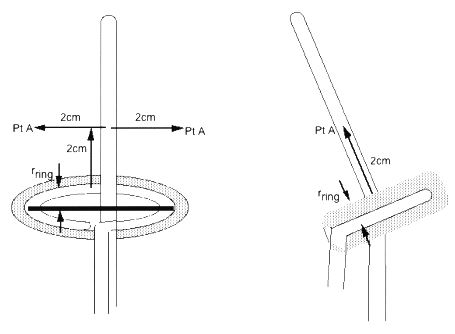
\includegraphics[width=0.43\textwidth]{Imagens/pontoAanel.JPG}
			}} \\ %
		\subfigure{
			\fcolorbox{DarkTurquoise}{white}{%
				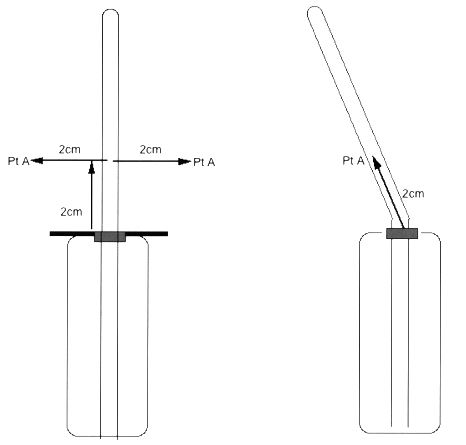
\includegraphics[width=0.44\textwidth]{Imagens/pontoAcilindrovazado.JPG}
			}} %
		\subfigure{
			\fcolorbox{DarkTurquoise}{white}{%
				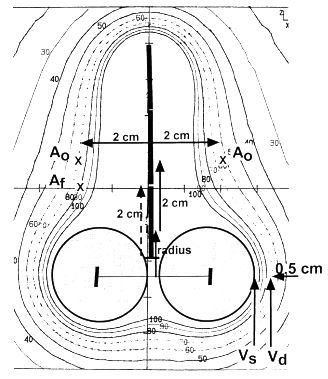
\includegraphics[width=0.36\textwidth]{Imagens/distribuicaoGuid.JPG}
			}} \\ %
		\caption{Determinação do Ponto A para diferentes aplicadores.}
		\label{fig:pontoA}
	\end{figure}

	Para definir o falloff lateral de dose, o sistema Manchester usa o \textcolor{DarkTurquoise}{\textbf{ponto B (esquerdo e direito)}} definido como: \textcolor{MediumOrchid}{\textit{No TPS, conecte uma linha através do centro de cada ovóide ou a posição de parada mais lateral em um anel. A partir do ponto no tandem onde esta linha se cruza, estenda superiormente o raio dos ovóides ou para os anéis mova-se superiormente até o topo do anel e depois mova 2 cm ao longo da linha média do paciente. Defina o ponto B em cada lado como 5 cm lateralmente em uma linha perpendicular a partir deste ponto na linha média do paciente}}. Observe que a linha que conecta os pontos B é sempre perpendicular à linha média do paciente, como mostra a \ref{fig:pontoB}.

	\begin{figure}[h]
		\centering
		\fcolorbox{DarkTurquoise}{white}{%
			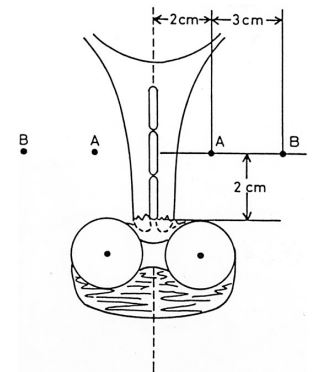
\includegraphics[width=0.4\textwidth]{Imagens/pontoB.JPG}
		}%
		\caption{Determinação do Ponto B e sua relação com o ponto A e com a linha média do paciente}
		\label{fig:pontoB}
	\end{figure}

	Dentro do sistema Manchester, diferentes padrões de carregamento (em LDR) ou tempo de parada (em HDR) podem ser usados para moldar a distribuição de dose. Portanto, o profissional deve estar ciente de que a mesma prescrição de dose para os pontos A não restringe a variação na distribuição de isodose em aproximadamente uma forma de pêra.

\subsection*{Guidelines para Contorno da ABS e ESTRO}

	O grupo GEC-ESTRO publicou um conjunto de diretrizes de contorno para câncer de colo de útero usando imagens de TC e RM. Para o tratamento definitivo usando uma combinação de EBRT e braquiterapia, a topografia variável requer uma imagem adaptativa e uma abordagem de contorno para o planejamento do tratamento de braquiterapia. O grupo GEC-ESTRO despendeu um esforço significativo estudando as diferentes abordagens de tratamento em quatro grandes centros europeus de braquiterapia e, após vários workshops intensivos, forneceu as seguintes recomendações para definições de volume:

	\begin{itemize}[label=\textcolor{CarnationPink}{$\blacksquare$}]
		\item O GTV contém o volume tumoral bruto visível conforme definido pelo ICRU-50, ICRU-62 e ICRU-83.
		\item O CTV de alto risco (HR-CTV) contém o colo do útero e qualquer doença macroscópica visível (GTV).
		\item O CTV de risco intermediário (IR-CTV) contém áreas de doença macroscópica inicial no início do tratamento, mas no momento do contorno apresenta no máximo extensão microscópica da doença. 
		\item O CTV de baixo risco (LR-CTV) abrange áreas potenciais para doença microscópica.
	\end{itemize}

	Esses volumes são ainda subdivididos pela extensão da doença no momento do diagnóstico (subscrito D) e em cada fração subsequente de braquiterapia (subscritos B1, B2, \dots).

	Todos os órgãos de risco devem ser contornados. Para braquiterapia ginecológica e geniturinária (GU), isso inclui o reto, o cólon sigmóide e a bexiga. O ABS recomenda avaliar $D_{2cc}$, $D_{0.1cc}$ e $D_{max}$ para cada órgão de risco. A ABS não faz uma recomendação específica para rastrear a dose nos linfonodos, mas admite que os pontos B (pontos da parede pélvica) definidos pelo ICRU-38 possam ser usados.

\subsection*{Planejamento de Tratamento e Algoritmos do TPS}

	No planejamento do tratamento, dois tipos de estratégias de planejamento podem ser usados:

	\begin{enumerate}
		\item Planos padrão; ou
		\item Planos personalizados.
	\end{enumerate}

	Os \textcolor{DarkTurquoise}{\textbf{planos padrão}} são recomendados apenas para uso em braquiterapia intracavitária baseada em cilindros, porque a linha de referência de prescrição é fixa em relação à geometria do aplicador seja na superfície do aplicador ou a 5 mm de distância da superfície do aplicador. Para criar um plano padrão, uma CT de um cilindro é criada e importada no sistema de planejamento de tratamento. Os planos de cilindro são caracterizados por:

	\begin{itemize}[label=\textcolor{CarnationPink}{$\blacktriangleright$}]
		\item Dose por fração;
		\item Diâmetro do cilindro, tipo de capa e número de segmentos. O tipo de capa determinará a cobertura superior. Para doenças mais extensas, pode ser desejável deslocar a dose mais para cima, e o uso de uma capa com uma posição de parada mais distal pode facilitar isso.
		\item Duração do tratamento;
		\item Localização da linha de prescrição (superfície do cilindro e/ou 5 mm de distância da superfície);
		\item Posição de parada e tempos de parada.
	\end{itemize}

	Os \textcolor{DarkTurquoise}{\textbf{Planos personalizados}} podem ser usados para cilindros e devem ser usados para todos os outros planos de tratamento intracavitário. Se um tratamento for administrado em um padrão fracionado, a localização do aplicador deve ser verificada por meio de uma imagem adquirida antes de cada fração. A colocação repetida do tandem é facilitada pela colocação de um stent uterino suturando-o no momento da primeira fração. Isso possibilita a colocação do aplicador para futuras frações sem o uso de anestesia. Os algoritmos de otimização de dose disponíveis para os TPS de HDR permitem uma flexibilidade consideravelmente maior na modelagem da dose em comparação com a braquiterapia LDR que apresenta um número limitado de fontes e  de intensidade da fonte.

	A ABS recomenda que os planos de tratamento para tratamentos de colo uterino (T\&O, T\&R, T\&C) devam conter e reportar os seguintes parâmetros:

	\begin{itemize}[label=\textcolor{CarnationPink}{$\blacktriangleright$}]
		\item Dose por fração e dose total;
		\item Tipo de aplicador;
		\item Radionuclídeo, incluindo a intensidade da fonte;
		\item Posição de parada e tempos de parada;
		\item Pontos de reto e da bexiga definidos no ICRu e/ou $D_{2cc}$, $D_{0.1cc}$ e $D_{max}$ para cada órgão de risco ($D_{5cc}$ para a parede do órgão, se for utilizada).
		\item Distribuições de isodose no plano sagital, coronal frontal oblíquo através dos pontos A e axial através das fontes vaginais.
	\end{itemize}

	A dose para órgãos críticos é tratada de forma diferente com base na área a ser tratada e no tipo de aplicador. A \ref{fig:criteriosBraqui} mostra alguns critérios nas configurações clínicas mais comuns.

	\begin{figure}[h]
		\centering
		\fcolorbox{DarkTurquoise}{white}{%
			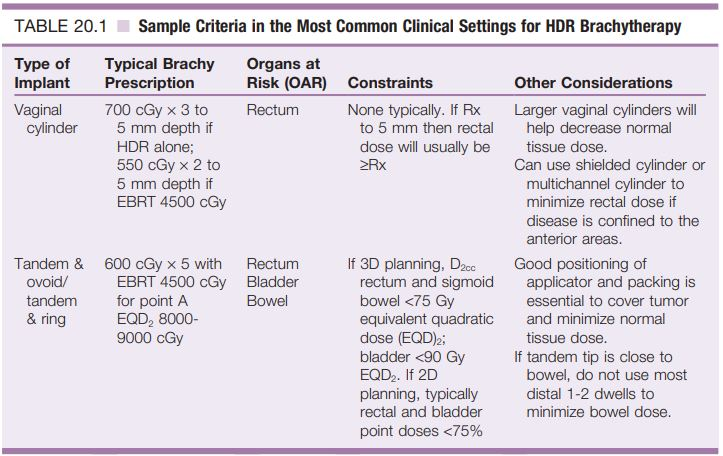
\includegraphics[width=0.7\textwidth]{Imagens/criteriosBraqui.JPG}
		}%
		\caption{Critérios nas configurações clínicas mais comuns para braquiterapia HDR}
		\label{fig:criteriosBraqui}
	\end{figure}

	A maioria dos TPS usa o formalismo AAPM TG-43 para cálculos de dose. Algoritmos de cálculo de dose baseados em modelos estão se tornando disponíveis. AAPM TG-186 sobre algoritmos de cálculo de dose baseados em modelos, recomenda reportar as doses e as prescrições de dose no formalismo AAPM TG-43 com os resultados de cálculo de dose baseados em modelo reportados além dos cálculos AAPM TG-43. Essa abordagem é análoga à abordagem do Radiation Therapy Oncology Group (RTOG) para implementar novos algoritmos de correção de heterogeneidade em tratamentos pulmonares: reportar os dois métodos em paralelo para garantir uma transição sistemática na prescrição de dose e permitir tempo para validação experimental e clínica completa do novo algoritmos de cálculo de dose.

	Existem várias técnicas utilizadas para o planejamento da braquiterapia HDR. No planejamento forward, os tempos de parada e as posições de parada podem ser definidos para simular os padrões de carregamento de um implante LDR. Deve-se notar que, embora as linhas de isodose pareçam idênticas àquelas alcançadas um implante LDR, a dose biologicamente equivalente (BED) em diferentes pontos do implante será diferente. O método de planejamento forward mais comum é começar com posições de parada e tempos de parada simulando um implante LDR e, em seguida, ajustar manualmente as posições de parada até que a forma da distribuição de dose desejada seja alcançada. Esta distribuição de dose é então normalizada para os pontos A (colo do útero) ou para a linha de referência para tratamentos de cilindros. Para implantes intracavitários usando contornos volumétricos baseados no GEC-ESTRO, o planejamento inverso pode ser usado para otimizar a cobertura de dose do HR-CTV. Além de reportar a dose para o volume, a dose para os pontos A, bem como a dose para os pontos retal e de bexiga do ICRU38, devem ser reportadas para dar continuidade aos sistemas tradicionais de prescrição de dose.


\section{Pontos Chave}

	A braquiterapia intracavitária está mudando cada vez mais de LDR para HDR devido a uma variedade de razões, incluindo menos exposição à radiação para funcionários com afterloaders remotos e menos tempo de internação para os pacientes. Ao comparar estudos de LDR versus HDR, é importante estar atento às conversões de dose equivalentes e aplicar padrões como EQD2. Para os sítios comuns que utilizam braquiterapia intracavitária, existem boas diretrizes da ABS e de outras sociedades.

	A braquiterapia intracavitária é frequentemente usada para tratar cânceres ginecológicos. Na braquiterapia com cilindro vaginal, é importante usar o maior diâmetro de cilindro que a paciente possa tolerar para diminuir a dose na superfície do cilindro e o risco de gaps de ar. Existem vários sistemas de cilindros, alguns com blindagem para proteção do tecido normal. Da mesma forma para o tratamento do câncer de colo de útero, vários sistemas podem ser usados para o tratamento T\&O, e os sistemas T\&R estão se tornando mais populares. A chave para um tratamento eficaz neste cenário é a boa colocação do T\&O/T\&R e o tamponamento para ajudar a estabilizar o aplicador e mover tecidos normais, como o reto, para longe da região de alta dose. Outras aplicações menos comuns da braquiterapia incluem cânceres uterinos inoperáveis, tumores endobrônquicos, tumores esofágicos e tumores da nasofaringe.

	O planejamento do tratamento baseado em TC ou RM é mais rotineiramente usado para ajudar a delinear o volume alvo e os tecidos normais. Tradicionalmente, a braquiterapia registra doses pontuais (como ponto A, ponto bexiga, ponto retal). O sistema Manchester foi usado para definir muitos dos pontos de interesse no planejamento tradicional e ainda está sendo usado. Com o planejamento 3D, fica claro que nem sempre esses pontos coincidem com a dose máxima no órgão. Os planos de isodose fornecem informações adicionais das doses pontuais ao avaliar os planos de tratamento, embora as diretrizes exatas para a avaliação do plano de isodose ainda estejam evoluindo. A ABS tem diretrizes para registro de parâmetros de tratamento. Para tratamentos simples, como um cilindro vaginal, um plano padrão pode ser usado porque a geometria do aplicador e a anatomia do paciente são fixas. Caso contrário, planos personalizados devem ser gerados para refletir a localização do aplicador em relação à anatomia local. Para tratamentos fracionados, a posição de aplicação deve ser verificada antes de cada fração.

	Os cálculos de dose estão melhorando para a braquiterapia, com a disponibilização de algoritmos baseados em modelos. Estes ainda precisam de mais validação, mas devem melhorar a precisão da dose no futuro.





\bibliography{ref.bib}
\end{document}